%! Author = zhiweizhang
%! Date = 10.06.25

\chapter{Model Deployment and \ac{API} Service}\label{chapter:model-deployment-and-api-service}

To facilitate real-world application and integration of the trained classification models, an \ac{API} service was
developed to serve the best-performing models from both the binary and multi-class classification tasks. The service
was designed with modularity, portability, and ease of use in mind.

Although the \ac{API} service was not deployed to an online hosting platform due to infrastructure constraints, it was
fully implemented, containerized using Docker, and published to Docker Hub. This approach ensures reproducibility
and allows collaborators (e.g., from the social science department) or third-party researchers to easily run the
service in local or cloud-based environments supporting Docker runtime.

\section{System Architecture}

~\autoref{fig:system-architecture} presents the system architecture of the classification \ac{API} service. Users
submit an image file via an HTTP request, which is then routed to one of three model pipelines based on the
specified task: binary classification, multi-class classification, or a two-stage hierarchical pipeline.

In the two-stage (or "2-layer") classification pipeline, the image is first passed to the binary classifier to
determine whether it contains Nazi symbolism. If the result is negative, the \ac{API} returns a response indicating the
absence of such symbols. If the binary classifier detects the presence of Nazi-related content, the image is
subsequently passed to the multi-class classifier, which identifies the specific type of Nazi symbol (e.g.,
swastika, \ac{SS} bolts, eagle).

This cascaded approach reduces unnecessary computation for images that do not contain relevant content and mirrors
real-world moderation workflows that apply more granular analysis only when initial filters are triggered.

The backend is implemented using \texttt{FastAPI}, and each model is preloaded into memory at service startup for
low-latency prediction. The architecture is stateless and containerized, making it suitable for horizontal scaling
in distributed environments.


\begin{figure}[ht]
    \centering
    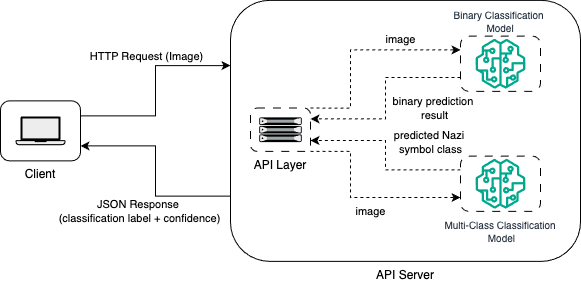
\includegraphics[width=0.7\textwidth]{figures/system_architecture}
    \caption{System architecture of the implemented classification \ac{API} service, including the 2-layer classification pipeline.}
    \label{fig:system-architecture}
\end{figure}

\section{Model Integration and Selection Logic}

To support different classification tasks, the \ac{API} service provides separate, clearly defined endpoints for binary
classification, multi-class classification, and the combined 2-layer classification pipeline. Rather than
dynamically selecting the model based on a request payload parameter, each endpoint is mapped to a specific inference pipeline.

This design simplifies both server-side logic and client-side usage, allowing users to directly call the appropriate
endpoint for their task without needing to specify a task identifier. Each endpoint handles all necessary
preprocessing, model loading, and prediction steps internally.

All models are preloaded into memory when the \ac{API} server starts. Models implemented using PyTorch are serialized with
\texttt{TorchScript} or saved in standard PyTorch format, while traditional machine learning models (e.g., logistic
regression or \ac{SVC} with OpenCLIP embeddings) are serialized using \texttt{joblib}. Loading models once at startup
significantly reduces runtime latency and avoids redundant I/O operations during each prediction request.

This modular design also makes the system extensible—new models or task-specific pipelines can be added by
registering additional routes in the \ac{API} codebase without impacting the existing ones.

The route-to-model mapping logic is summarized in ~\autoref{fig:api-model-routing}, which shows how each \ac{API}
endpoint corresponds to a specific classification pipeline.

%! Author = zhiweizhang
%! Date = 11.06.25

% Preamble
\begin{figure}[ht]
\centering
\resizebox{\textwidth}{!}{
\begin{tikzpicture}[
    node distance=1.5cm and 2cm,
    every node/.style={font=\small},
    process/.style={rectangle, draw=blue!50, fill=blue!10, thick, minimum width=3.5cm, minimum height=0.9cm},
    endpoint/.style={rectangle, draw=black!80, fill=gray!10, thick, minimum width=4cm, minimum height=0.9cm},
    decision/.style={diamond, aspect=2, draw=red!60, fill=red!10, thick, minimum height=1.2cm},
    response/.style={rectangle, draw=green!50!black, fill=green!10, thick, minimum width=3.5cm, minimum height=0.9cm},
    arrow/.style={->, thick}
]

% API Endpoints
\node[endpoint] (binary) {POST /predict-binary};
\node[endpoint, below=of binary] (multi) {POST /predict-multiclass};
\node[endpoint, below=of multi] (twolayer) {POST /predict};

\node[process, right=of multi] (prep) {Image Preprocessing};

% Two-layer path
\node[decision, right=of prep] (decision) {Contains Nazi Symbol?};
\node[process, right=of decision] (negresponse) {Return: No Symbol};

% Binary path
\node[process, above=2cm of decision] (binarymodel) {Binary Classifier};
\node[response, right=of binarymodel] (binaryresp) {Binary Prediction Response};

% Multi-class path
\node[process, below=2cm of decision] (multimodel) {Multi-Class Classifier};
\node[response, right=of multimodel] (multiresp) {Multi-Class Prediction Response};

\node[response, below right=of multimodel] (finalresp) {Hierarchical Prediction Response};
% Arrows
\draw[red, arrow] (binary.east) -| (prep.150);
\draw[red, arrow] (prep.north) |- (binarymodel.west);
\draw[red, arrow] (binarymodel) -- (binaryresp);

\draw[blue, arrow] (multi) -- (prep);
\draw[blue, arrow] (prep.south) |- (multimodel.west);
\draw[blue, arrow] (multimodel) -- (multiresp);

\draw[arrow] (twolayer.east) -| (prep.-150);
\draw[arrow] (prep) -- (binarymodel);
\draw[arrow] (binarymodel) -- (decision);
\draw[arrow] (decision) -- node[above right] {No} (negresponse);
\draw[arrow] (decision) -- node[below right] {Yes} (multimodel);
\draw[arrow] (multimodel.south) |- (finalresp.west);

\end{tikzpicture}
}
\caption{\ac{API} endpoints mapped to model pipelines, including the 2-layer classification logic.}
\label{fig:api-model-routing}

\end{figure}

\section{Continuous Integration and Deployment}

The service is fully integrated with a GitHub Actions \ac{CI/CD} pipeline, as shown in ~\autoref{fig:github-pipeline}.
This pipeline automates the following tasks:

\begin{itemize}
    \item Code quality checks and unit testing.
    \item Building and tagging of Docker images.
    \item Publishing Sphinx-based documentation to GitHub Pages.
    \item Pushing the Docker image to Docker Hub.
\end{itemize}

Although the final service is not deployed to a live endpoint, the \ac{CI/CD} pipeline ensures that each commit to the
main branch triggers a build and test process, ensuring long-term maintainability. Users can reliably pull the
latest image version and run it locally or deploy it on a remote host with minimal setup.

\begin{figure}[ht]
    \centering
    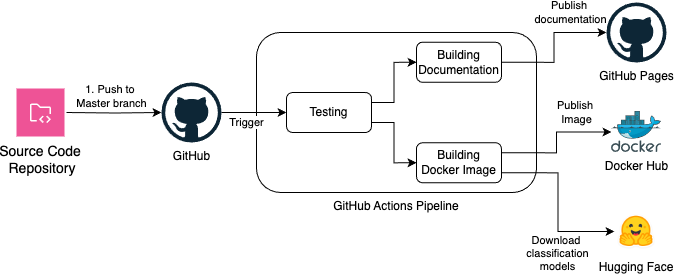
\includegraphics[width=0.7\textwidth]{figures/github_pipeline}
    \caption{GitHub Actions \ac{CI/CD} pipeline for Dockerized \ac{API} service.}
    \label{fig:github-pipeline}
\end{figure}

\section{\ac{API} Endpoints}

The \ac{REST} \ac{API} exposes several endpoints to support classification, health checks, and automatic documentation.
~\autoref{tab:api-endpoints} provides an overview of the available endpoints.

In addition to individual endpoints for binary and multi-class classification tasks, the \ac{API} includes a dedicated
endpoint for the 2-layer classification workflow. This endpoint abstracts the logic of cascading model inference: it
first applies the binary classifier and, only if Nazi symbolism is detected, invokes the multi-class model to
provide a more specific label.

This design simplifies client-side logic and makes it easier to embed the classifier into larger moderation or
research pipelines without needing to handle the decision tree manually.

%! Author = zhiweizhang
%! Date = 10.06.25

% Preamble
\begin{table}[ht]
  \centering
  \resizebox{\textwidth}{!}{
  \begin{tabular}{llp{8cm}}
    \toprule
    \textbf{Method} & \textbf{Endpoint} & \textbf{Description} \\
    \midrule
    \texttt{POST}   & \texttt{/predict} & Runs the 2-layer pipeline: binary classification followed by multi-class prediction if Nazi content is detected. Threshold for symbol inclusion is 0.1. \\
    \texttt{POST}   & \texttt{/predict-binary} & Performs binary classification with associated confidence scores. \\
    \texttt{POST}   & \texttt{/predict-multiclass} & Performs multi-label classification of Nazi symbol types. Returns predictions above confidence threshold 0.1. \\
    \texttt{GET}    & \texttt{/health} & Health check endpoint. \\
    \texttt{GET}    & \texttt{/version} & Returns model and \ac{API} version metadata. \\
    \texttt{GET}    & \texttt{/docs} & Serves OpenAPI documentation via Swagger UI. \\
    \bottomrule
  \end{tabular}
  }
  \caption{Summary of available \ac{API} endpoints.}
  \label{tab:api-endpoints}
\end{table}

All classification endpoints accept images as multipart form data and return structured \ac{JSON} responses. These
responses include predicted class labels, confidence scores, and metadata about the model used. The \ac{API} is
documented using OpenAPI and is accessible via the \texttt{/docs} route.

\subsection{Example \ac{JSON} Response: Binary Classification}
The \ac{API} returns predictions in \ac{JSON} format. An example response for the binary classification endpoint is shown below:

\begin{figure}[ht]
\centering
\begin{lstlisting}[language=json]
[
  {
    "prediction": "nazi",
    "confidence": 0.965,
  }
]
\end{lstlisting}
\caption{Sample \ac{JSON} response for binary classification prediction.}
\end{figure}

\subsection{Example \ac{JSON} Response: Multi-Class Classification}
For multi-class classification, the \ac{API} returns all predicted classes with probability above the threshold ($\geq 0.1$).

\begin{figure}[ht]
\centering
\begin{lstlisting}[language=json]
{
  "nazi_symbols": ["swastika", "siegrune", "black_sun"],
  "details": [
    {"label": "swastika", "confidence": 0.882},
    {"label": "siegrune", "confidence": 0.062},
    {"label": "black_sun", "confidence": 0.016}
  ],
}
\end{lstlisting}
\caption{Sample \ac{JSON} response for multi-class classification prediction.}
\end{figure}

\subsection{Example \ac{JSON} Response: 2-layer Classification}
This endpoint combines binary and multi-class classification. It first predicts whether the image contains Nazi
symbols, then returns all matching symbols above the confidence threshold.

\begin{figure}[ht]
\centering
\begin{lstlisting}[language=json]
{
  "containing_nazi_symbols": true,
  "prob": 0.97,
  "nazi_symbols": ["swastika", "siegrune", "black_sun"],
  "details": [
    {"label": "swastika", "confidence": 0.882},
    {"label": "siegrune", "confidence": 0.062},
    {"label": "black_sun", "confidence": 0.016}
  ]
}
\end{lstlisting}
\caption{Sample \ac{JSON} response for 2-layer classification prediction.}
\end{figure}

\subsection{Thresholding vs. Top-$k$ in Multi-label Classification}

In the multi-class classification task, an image may contain more than one Nazi symbol, making it inherently a
multi-label problem. Instead of using a top-$k$ prediction strategy, where the model returns the $k$ most confident
classes regardless of their absolute probabilities, a fixed probability threshold of 0.1 was used to filter
predicted classes.

The thresholding approach offers two key advantages in this context:

\begin{enumerate}
    \item \textbf{Adaptability to Varying Symbol Counts}: Since different images may contain a varying number of
    symbols—including just one or many—the threshold-based method allows the model to return a flexible number of
    predictions based on actual confidence levels. In contrast, a top-$k$ method would always return a fixed number
    of classes, potentially introducing irrelevant or low-confidence predictions.

    \item \textbf{Minimization of False Positives}: By applying a threshold (empirically chosen as 0.1), the system
    filters out low-probability predictions, thereby reducing the risk of returning implausible or incorrect symbol
    classifications. This is especially important in a sensitive domain such as Nazi symbol detection, where false
    positives can have serious implications.
\end{enumerate}

This threshold-based multi-label design more accurately reflects the real-world complexity of the task and aligns
with the goal of precise and responsible detection of harmful content.



\section{Extensibility and Future Deployment}

The \ac{API} service is designed with modularity and extensibility in mind. New classification tasks—such as object
detection for symbol localization, \ac{OCR}, or broader hate symbol recognition—can be integrated by registering
additional model pipelines and endpoints. Thanks to the decoupled routing logic and preloading of models, such
extensions require minimal code changes.

Although the service is not deployed online, it is fully containerized and prepared for local or remote deployment.
The GitHub repository includes:

\begin{itemize}
    \item A \texttt{Dockerfile} and \texttt{pyproject.toml} to ensure consistent environments
    \item Usage instructions for running the service locally via \texttt{docker run} or \texttt{docker-compose}
    \item Example requests (e.g., \texttt{curl} commands) and a Postman collection for testing
    \item CI pipelines using GitHub Actions for testing, documentation, and Docker image publishing
\end{itemize}

This setup ensures reproducibility and ease of use for collaborators such as the social science chair, who can
launch the service locally with no additional configuration. All models are preloaded at startup, avoiding runtime
delays or dependency mismatches.

In future iterations, the service could be deployed to cloud platforms such as AWS, Google Cloud, or Azure, using
container orchestration tools like Kubernetes or serverless options like AWS Lambda with \ac{API} Gateway. To support
public or production-level access, additional features such as user authentication, input rate-limiting, and secure
storage of logs and models would be required.

This flexible and portable design ensures that the system can evolve alongside the research project and scale into
production-oriented or collaborative infrastructures as needed.

